\header[h]{
    \headtitle{Belle Eugénie} \label{belle-eugenie}
    %
    \insertComment{}{}
}

\enluminure{2}{\href{}{B}}{elle Eugénie} tu dors bien à ton aise
\\Tu ne sais pas ce que l'on dit de toi
\\\\On dit de toi que tu n'es pas sincère
\\Tu as charmé le coeur d'un officier
\\\\Si j'l'ai charmé que veux-tu que j'y fasse
\\Tous mes parents me défendent de t'aimer
\\\\Si tes parents te défendent cette chose
\\Ecoute-les, mais ne m'en parle plus
\\\\Pour moi j'irai dans un bois solitaire
\\Finir mes jours sous l'ombre d'un rocher
\\\\Sous le rocher y'a une fontaine
\\Le rossignol y chante nuit et jour
\\\\Et il nous dit dans son joli langage
\\Les amoureux sont souvent malheureux.

\vspace{0.5cm}
\begin{figure}[h!]
\centering
   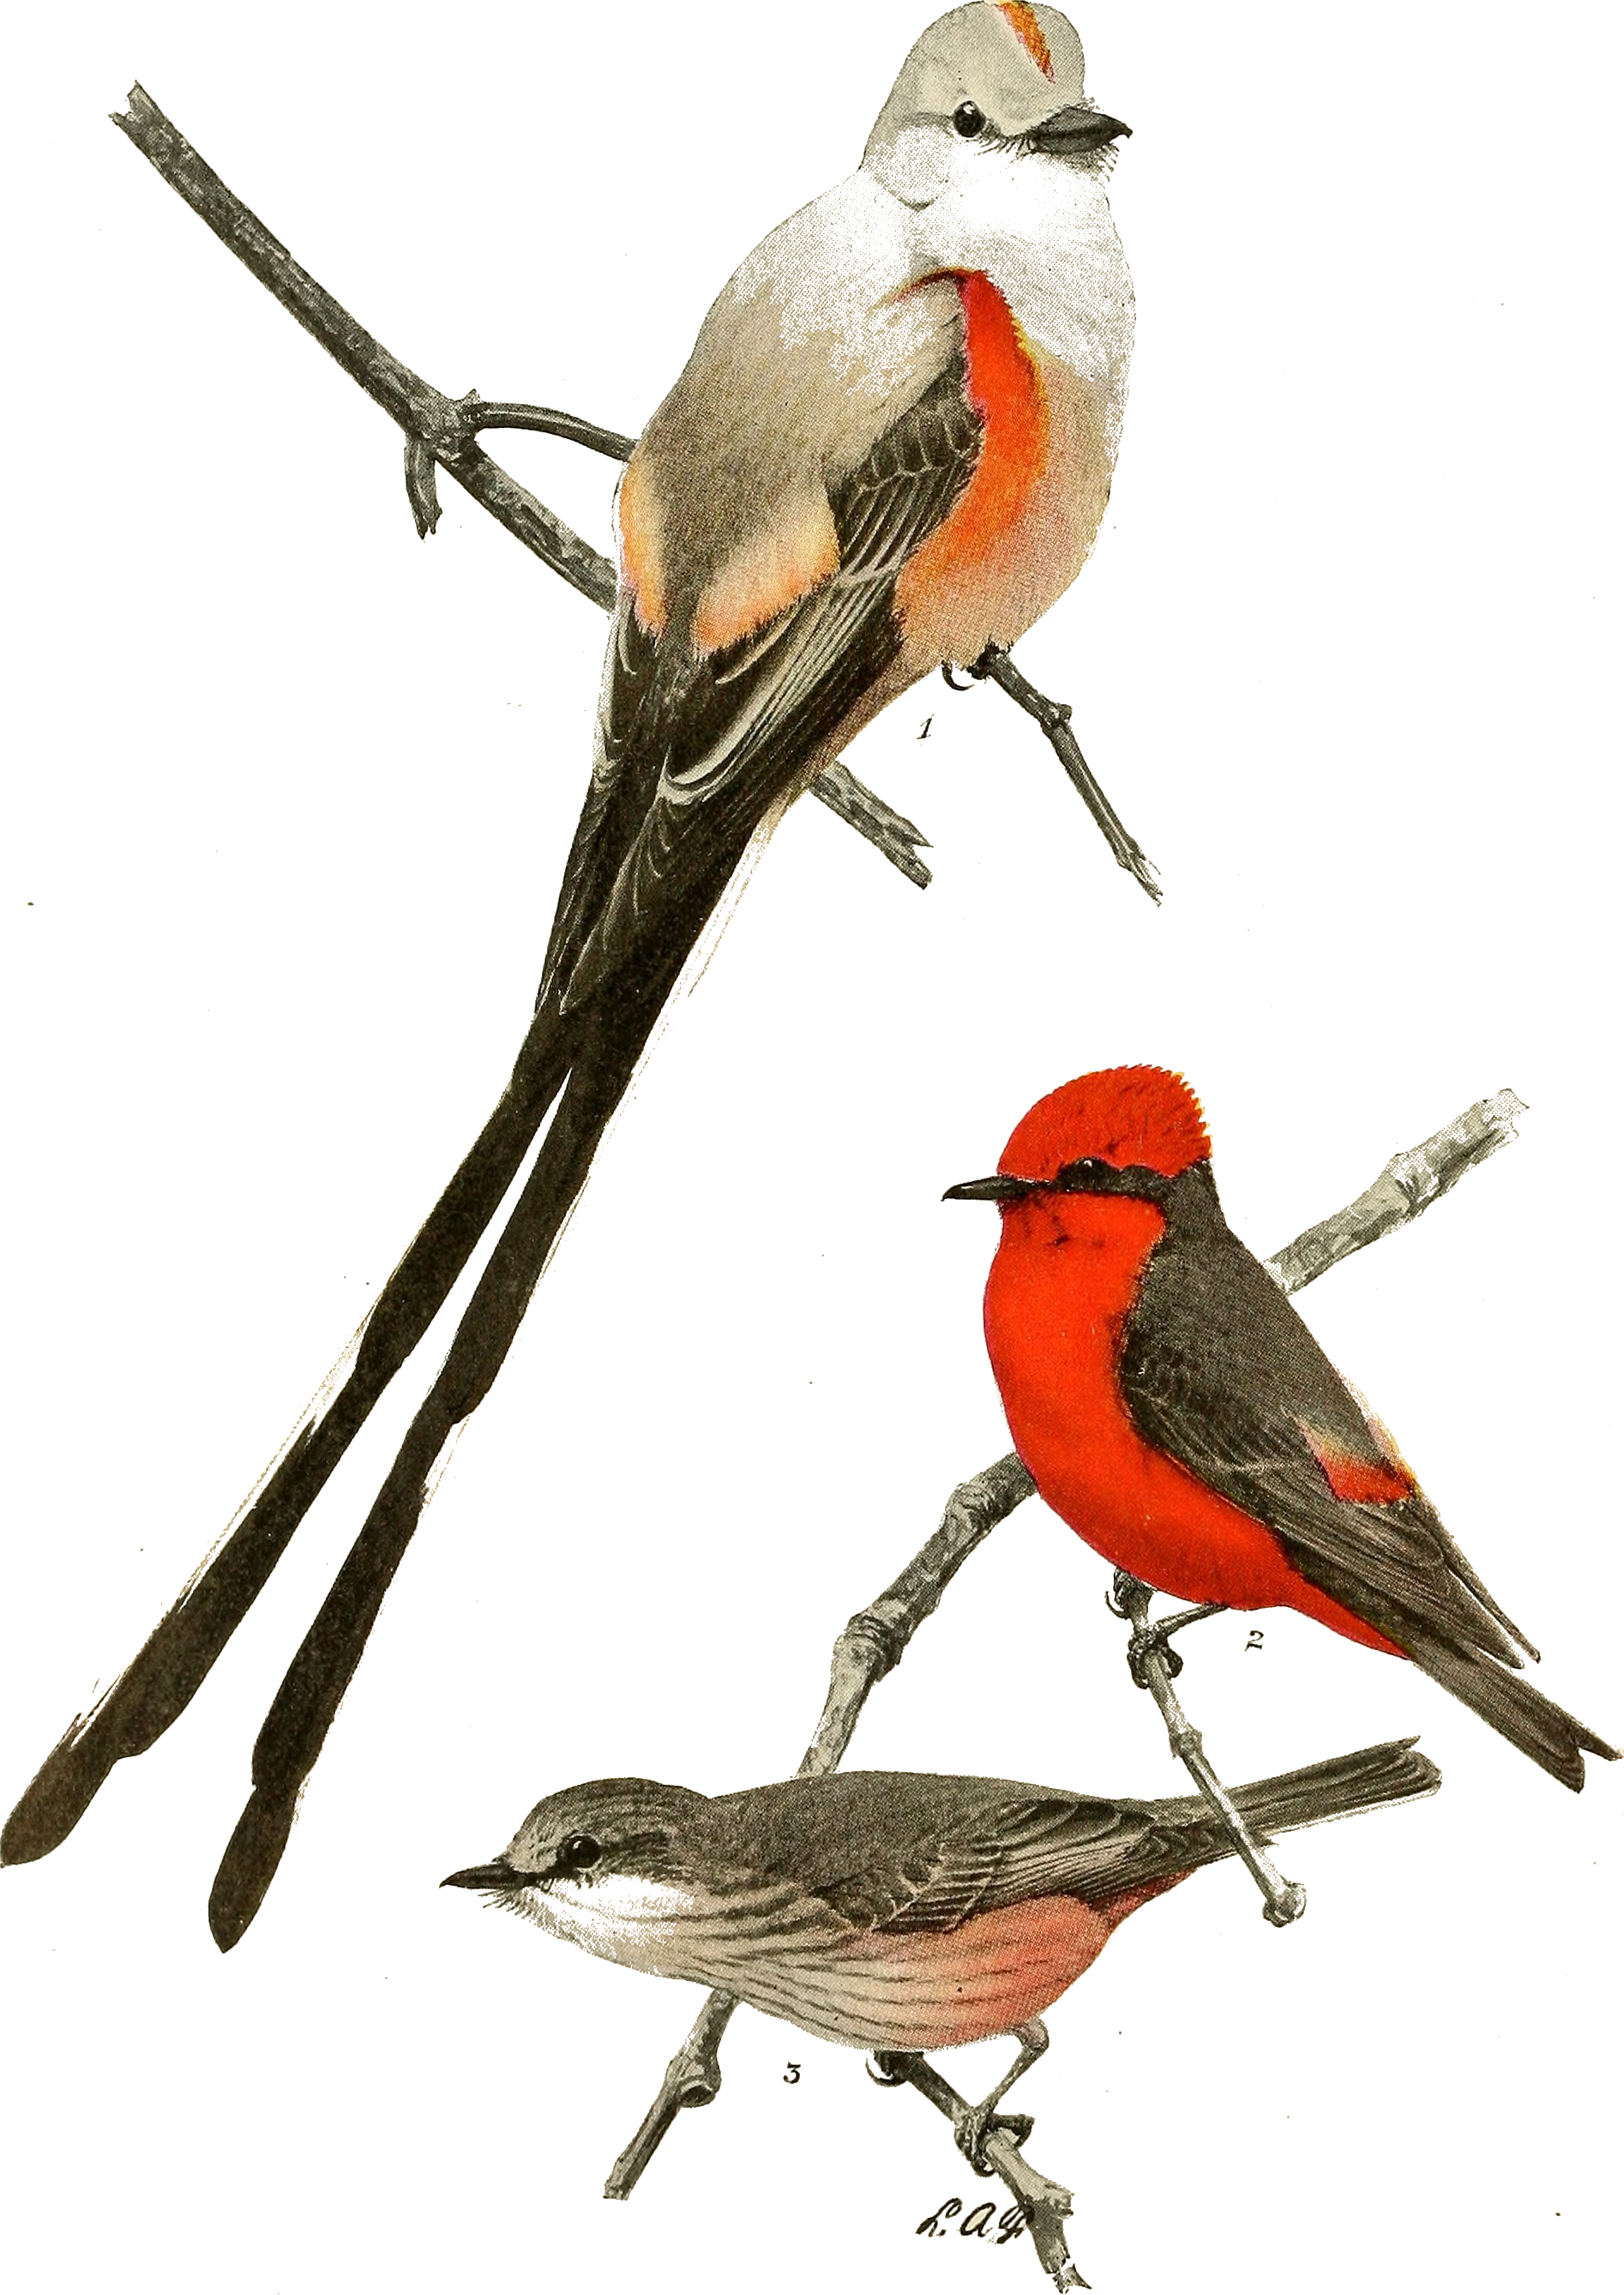
\includegraphics[width=0.4\textwidth]{images/brev61.png}
 \end{figure}


\breakpage